\documentclass[a4paper,11pt]{report}

\usepackage[utf8]{inputenc}
\usepackage[italian]{babel}
\usepackage{amsmath}
\usepackage{amsfonts}
\usepackage{xfrac}
\usepackage{hyperref}

\usepackage{amsmath}
\usepackage{array}
\usepackage{amstext}
\usepackage{amsthm}
\usepackage{enumitem}
\usepackage{fancyhdr}
\usepackage{eurosym}
\usepackage{amsmath,amssymb}
\usepackage{graphicx}

\hypersetup{
    colorlinks=false,
    pdfborder={0 0 0},
}

\usepackage{listings}
\usepackage{lstautogobble}

\lstset{basicstyle=\ttfamily,
  mathescape=true,
  escapeinside=||,
  autogobble}
  
\setlength{\parindent}{0pt}

\newcommand{\der}[2]{\frac{\delta #1}{\delta #2}}
\newcommand{\dder}[2]{\frac{\delta^2 #1}{\delta #2^2}}
\newcommand{\dmix}[3]{\frac{\delta^2 #1}{\delta #2 \delta #3}}

\newtheorem{definition}{Definizione}[chapter]
\newtheorem{theorem}{Teorema}[chapter]
\newtheorem{prop}{Proposizione}[chapter]
\newtheorem{lem}{Lemma}[chapter]
\theoremstyle{osservazione}
\newtheorem{osservazione}{Osservazione}[chapter]
\theoremstyle{esempio}
\newtheorem{esempio}{Esempio}[chapter]
\theoremstyle{notazione}
\newtheorem{notazione}{Notazione}[chapter]
\theoremstyle{corollario}
\newtheorem{corollario}{Corollario}[chapter]

\begin{document}

\thispagestyle{empty}

	\begin{center}
	 {\large{\textbf{POLITECNICO DI MILANO}\\
             Corso di Laurea Magistrale di Ingegneria Matematica\\
             Facolt\`a di Ingegneria dei Sistemi\\
             }}
	\end{center}

	\vspace{1cm}
	\begin{figure}[htbp]
	\begin{center}
	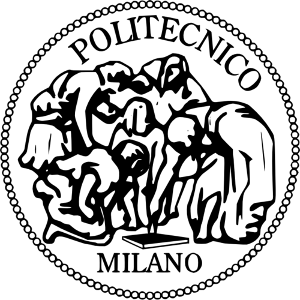
\includegraphics[width=4cm]{img/poli_logo.png}
	\end{center}
	\end{figure}
	
	\vspace{1cm}
	\begin{center}
	{\LARGE{Progetto di Programmazione Avanzata per il Calcolo Scientifico:}}
	\end{center}
	%\color{white}
	\vspace{2cm}
	\begin{center}
	{\LARGE{\textbf{Option Pricing per modelli Exponential-L\'evy in 1d e 2d.}}}
	\end{center}
	
	%\color{black}
	%\vspace{2.5 cm}
	\begin{table}[hb!]
	\begin{center}
	\begin{tabular}{p{8cm}p{7cm}}
	& \\
  	& \\
  	& {\large Nahuel Foresta, matr. 798775}\\
	& {\large Giorgio G. Re, matr. 799260}\\
	\end{tabular}
	\end{center}
	\end{table}
	\begin{center}
	\vspace{3cm}
	\large{Anno Accademico 2012-2013}
	\end{center}

	\clearpage
	\thispagestyle{empty}
	
	\clearpage


\tableofcontents

\setcounter{secnumdepth}{0}

\chapter{Introduzione}

\chapter{Modello di Black \& Scholes}

\section*{Introduzione}
In questo capitolo descriviamo i modelli basilari utilizzati per descrivere il mercato finanziario, seguendo le argomentazioni di Merton (1973). Consideriamo quindi un mercato finanziario molto semplificato, costituito da un titolo \emph{risk-free} descritto dal processo $B$ e un titolo azionario con valore pari al processo $S$. Definiamo quindi questi due processi.
\begin{definition}
Sia $(\Omega,\mathcal{F},\mu)$ uno spazio misurabile e sia $\mathcal{F}_{t\in [ 0,T ]}$ una filtrazione. Allora, il processo B descrive il valore di un titolo \emph{risk-free} se la sua dinamica \`e del tipo: $$dB(t)=r(t)B(t)dt,$$dove $r$ \`e un qualsiasi processo $\mathcal{F}_t$-adattato.
\end{definition}
La caratteristica pi\`u importante quindi dei processi \emph{risk-free} \`e l'assenza del termine $W(t)$, ovvero l'assenza di aleatoriet\`a data da un moto browniano. Integrando infatti l'equazione precedente, otteniamo $$B(t)=B(0)\int_0^tr(s)ds.$$ Un caso particolare \`e quello in cui $r$ \`e una costante deterministica, in tal modo $B$ descrive l'andamento di un'obbligazione.
\\Assumiamo inoltre che la dinamica di $S$ sia data da: $$dS(t)=S(t)\alpha(t,S(t))dt+S(t)\sigma(t,S(t))dW(t),$$ in cui $W_t$ \`e un processo di Wiener (cio\`e, un moto browniano) e $\alpha$ e $\sigma$ due funzioni deterministiche. La funzione $\sigma$ \`e detta volatilit\`a del titolo, $\alpha$ \`e il \emph{local mean rate of return} ?!?!? di $S$.
\begin{osservazione}
Osserviamo la differenza fra il tasso di ritorno di un titolo \emph{risk-free} e quello di un titolo rischioso. Il tasso di $B$ \`e: $$\frac{dB(t)}{B(t)dt}=r(t),$$ ovvero totalmente deterministico, mentre quello di $S$ \`e dato da: $$\frac{dS(t)}{S(t)dt}=\alpha{t,S(t)}+\sigma \frac{dW(t)}{dt},$$ oggetto che non \`e osservabile al tempo $t$. Esso \`e infatti costituito dato da $\alpha$ e $\sigma$ che sono entrambi osservabili al tempo $t$, pi\`u un rumore bianco $W(t)$ che \`e del tutto casuale. Quindi, al contrario del titolo \emph{risk-free}, l'azione ha un tasso di ritorno stocastico, anche su una scala infinitesima.
\end{osservazione}
Passiamo ora a definire il modello di \emph{Black\&Scholes}.
\begin{definition}
Il modello di \emph{Black\&Scholes} consiste di due titoli con le seguenti dinamiche:
\begin{align}
dB(t)&=B(t)r(t)dt,\\
dS(t)&=\alpha S(t)dt+\sigma S(t)dW(t),
\end{align}
dove $r$, $\alpha$ e $\sigma$ sono costanti deterministiche.
\end{definition}

\section{Strumenti derivati e Opzioni}
In questa sezione definiamo gli strumenti derivati e, in particolare le opzioni che abbiamo trattato nel progetto.
\begin{definition}
In finanza, \`e denominato strumento derivato ogni contratto o titolo il cui valore si basa sul valore di mercato di un altro titolo o strumento finanziario, detto sottostante (ad esempio, azioni, valute, tassi di interesse o derivati stessi).
\end{definition}
Definiamo ora il titolo derivato pi\`u semplice, ovvero l'opzione \emph{call} europea.
\begin{definition}
Un'opzione \emph{call} europea con prezzo di esercizio (o \emph{strike price}) $K$ e scadenza $T$ sul sottostante $S$ \`e un contratto finanziario derivato con le seguenti caratteristiche:
\begin{itemize}
\item il titolare del contratto ha, al tempo $T$, il diritto di acquistare un'azione del sottostante al prezzo $K$ dal sottoscrittore del contratto, qualsiasi sia il valore del sottostante $S$ al tempo $T$;
\item il titolare del contratto non ha alcun obbligo di acquistare un'azione del sottostante al tempo $T$;
\item il diritto di acquistare un'azione del sottostante pu\`o essere esercitato solo al tempo $T$.
\end{itemize}
\end{definition}
\end{document}
